\documentclass{article}

% if you need to pass options to natbib, use, e.g.:
% \PassOptionsToPackage{numbers, compress}{natbib}
% before loading nips_2018

% ready for submission
\usepackage[final]{nips_2018}

% to compile a preprint version, e.g., for submission to arXiv, add
% add the [preprint] option:
% \usepackage[preprint]{nips_2018}

% to compile a camera-ready version, add the [final] option, e.g.:
% \usepackage[final]{nips_2018}

% to avoid loading the natbib package, add option nonatbib:
% \usepackage[nonatbib]{nips_2018}

\usepackage[utf8]{inputenc} % allow utf-8 input
\usepackage[T1]{fontenc}    % use 8-bit T1 fonts
\usepackage{hyperref}       % hyperlinks
\usepackage{url}            % simple URL typesetting
\usepackage{booktabs}       % professional-quality tables
\usepackage{amsfonts}       % blackboard math symbols
\usepackage{nicefrac}       % compact symbols for 1/2, etc.
\usepackage{microtype}      % microtypography
\usepackage{graphicx}
\usepackage{caption}
\usepackage{subcaption}
\usepackage{diagbox}
\usepackage{amsmath}
\graphicspath{{./img/}}

\title{Iterated Communication Through Negotation}

% The \author macro works with any number of authors. There are two
% commands used to separate the names and addresses of multiple
% authors: \And and \AND.
%
% Using \And between authors leaves it to LaTeX to determine where to
% break the lines. Using \AND forces a line break at that point. So,
% if LaTeX puts 3 of 4 authors names on the first line, and the last
% on the second line, try using \AND instead of \And before the third
% author name.

\author{
  Michael~Noukhovitch\\
  MILA\\
  \texttt{michael.noukhovitch@umontreal.ca} \\
}

\begin{document}

\maketitle

\begin{abstract}
    Recently, \cite{cao2018emergent} investigated the emergence of language in a
    negotiation game setting. We take a critical look at the setup, execution,
    and conclusions of this work. We note several drawbacks and missteps, and
    extend the work by correcting for them and updating the conclusions of this
    very interesting direction.
\end{abstract}

\section{Introduction}

One of the first philosophers of language, Ludvig Wittgenstein, posited that
"language is use" \cite{wittgenstein2009philosophical}. This idea, that the use
of language is what gives it its meaning, is a profound statement that also has
consequences for how we think of language. Wittgenstein saw language as wholly
tied to its use, there could be no language separate from reality or possible
use. To this end, he defined language games as games with simpler forms of
language "consisting of language and the actions into which it is woven".

Recently, the AI community has taken this philosophy of language and sought to
use it as the basis for the communication of autonomous agents
\cite{wagner2003progress}. The field of "emergent communication" seeks to
understand language starting from the most basic of language games; the goal is
to teach agents to communicate with each other by grounding their language and
interactions in a simpler world described by some "game." This game can be as
simple as two agents meeting at some point in a gridworld
\cite{goldman2007learning} to something as complicated as self-driving car
interactions \cite{resnick2018vehicle}.

In their ICLR paper, \cite{cao2018emergent} look at a negotiation game as the
basis of their investigation of emergent communication. The game involves two
agents $A$, and $B$ who seek to divide a pool of items $p$. Each agent has a
hidden utility over the items $u$ and the agents take turns creating proposals
$P$ of how to split the pool between themselves (e.g. if there are 5 of item 1,
an agent can suggest to split the pool 4 to themselves and 1 to the opponent).
Once an agent accepts their opponents proposal, agents recieve a reward given
their type: selfish agents $i$ only care about themselves and recieve a reward of
$u_i \cdot P$, whereas prosocial agents care equally about their opponent
and recieve reward $0.5 (u_A \cdot P + u_B \cdot P)$. Agents can communicate
across two possible channels during the game, the \textit{proposal channel}
where they can inform their opponent about their proposal, and the
\textit{linguistic channel} where agents can send a sequence of discrete
symbols. \cite{cao2018emergent} find that prosocial agents learn to use the
linguistic channel and perform better, whereas selfish agents do not and perform
worse. They posit that sociality may be a necessary trait for communication to
emerge.

\section{Related Work}%
\label{sec:related_work}

The negotiation game is a classical example of a zero-sum game from game theory
\cite{nash} but the approach to solving it is based off of recent work on
cooperative multi-agent reinforcement learning (MARL) \cite{panait}. This MARL
approach test the linguistic idea that cooperation is necessary for language
emergence \cite{nowak1999evolution} in the familiar context of emergent language
RL \cite{wagner2003progress}, but augmented with deep RL
\cite{laziridou2016multi}.


\section{Reproduction and Criticism}%
\label{sec:reproduction}

\subsection{Reproduction}%
\label{sub:reproduction}
The reproduction code is an extension of Hugh Perkins' attempt at reproducing
the paper \url{https://github.com/ASAPPinc/emergent_comms_negotiation} with
many notable fixes and extensions. The paper itself is relatively reproducible
with prosocial agent results being stronger than selfish agent results. And
prosocial agents using language as well as proposal being more successful than
agents just using proposals. The exact numbers achieved were not replicated,
neither were the results that prosocial agents with just a linguistic channel
achieved the highest score. Selfish agents in general tended to take longer to
converge and also had higher variance in their end result.

Reproducibility was not greatly hampered by resources as the code is not very
intensive but each full 500k episode run (with batch size 128) does take at
least 10 hours on a reasonable GPU. This means that reproducing the 10 run
average result and verifying any changes in a resilient way is probably only
feasible with access to a GPU cluster though there is quite a bit of room for
speedups.

\subsection{Criticism}%
\label{sub:criticism}

After reproducing results, there are still questions that are raised not about
the results themselves but about methodology and approach. We investigate some
of these questions.

\subsection{Prosocial Agents Don't Negotiate}%
\label{sub:prosocial_agents_don_t_negotiate}
A negotiation game where the interests of two parties do not clash is not as
much about negotiation as it is just sharing preferences and calculating the
optimum. This is exactly what is seen in case of prosocial agents with only a
linguistic channel: one agent communicates their preferences and the other
agent finds the optimal division and proposes it. In this way, the goal and even
the whole task is completely different for prosocial agents compared to selfish
agents whose selfish opponents do not have their best interests in mind. In this
way, selfish agents have no incentive to communicate their preferences as it
could potentially weaken their negotiating ability. In this way, we see that it
is not selfish agents failing to learn to communicate but learning to not
communicate not because they are selfish but because the situation does not
incentivise them to in a one-shot environment. This is explored in
\ref{sub:utility_channel}


\subsection{Unmotivated Agents}%
\label{sub:unmotivated_agents}
The paper and unfinished repository both allow for sampling situations that give
no possible reward to an agent, either through sampling a pool with 0 objects of
any kind or sampling a utility for an agent such that there are no object for
which they have non-zero utility (e.g. [1,0,1]). In this case, any rational
agent will accept any opponent's offer and there is no motivation to negotiate.
As well, if both agents are unmotivated then \textit{joint reward optimality}
of \cite{cao2018emergent} will be $\frac{0}{0}$.

\subsection{Fractional Reward is Biased}%
\label{sub:fractional_reward_is_biased}
The metric used by the paper "fraction of joint reward" compares the reward
achieved by each agent (utility over the accepted proposal $u_i \cdot P$) with
the total reward possible. In the case of prosocial
agents the metric measures the optimality as both agents' rewards are the same (
an equally weighted sum of their individual rewards) and they seek to optimize
the total possible reward.

\begin{equation}
    FR_{\text{prosocial}} = \frac{u_A \cdot P + u_B \cdot P}{\max u_A \cdot P + u_B \cdot P}
\end{equation}
\begin{align*}
    \text{where } u & \text{ is utility} \\
                  p & \text{ is the accepted proposal} \\
\end{align*}

This reward scheme is extended to selfish agents in \cite{cao2018emergent}.
But in the case of selfish agents, the total possible reward is the not the
objective the agent is optimizing. The agents optimize their own reward and
using the total possible reward metric is therefore a bad way of judging
performance, and inaccurate for judging an agent's negotiation ability.
Instead, you could measure how well each agent does at maximizing
their own reward, average across agents, and divide by the total possible reward

\begin{equation}
    FR_{\text{selfish}} = 0.5 * \frac{u_A \cdot P}{\max u_A \cdot P} + 0.5 * \frac{u_B \cdot P}{\max u_B \cdot P}
\end{equation}

But this is also wrong because the maximum possible reward for one agent will
usually decrease the reward for the opponent. In this way, the only situation where
$FR_{\text{selfish}} = 1$ is possible is if there do not exist any items for
which both agents have a non-zero utility. Since this situation is quite rare
(the whole point of negotiation is to resolve conflicting preferences) this
metric is unfair to selfish agents by usually being lower than for prosocial
agents and artificially makes them appear worse. Total possible reward is
therefore a bad metric for selfish agents and using a different metric is
proposed in \ref{sub:equitable_reward_metric}

\section{Exploratory Extensions}%
\label{sec:exploratory_experiments}

\subsection{Utility Channel}%
\label{sub:utility_channel}
One way to test whether selfish agents are learning to communicate or whether
they are specifically learning not to communicate is to simulate what
information an agent could possibly communicate. Since the prosocial agents
learn to communicate their hidden utilites, it seems fitting to test if giving
full information of hidden utilities helps achieve better
results. To this end, we experiment with giving an agent information about the
opponent's utility similar to a communication channel and plot agents' rewards
in fig \ref{fig:self-opp-util}.

\begin{figure}[h]
    \centering
    \begin{subfigure}{.5\textwidth}
    \begin{center}
        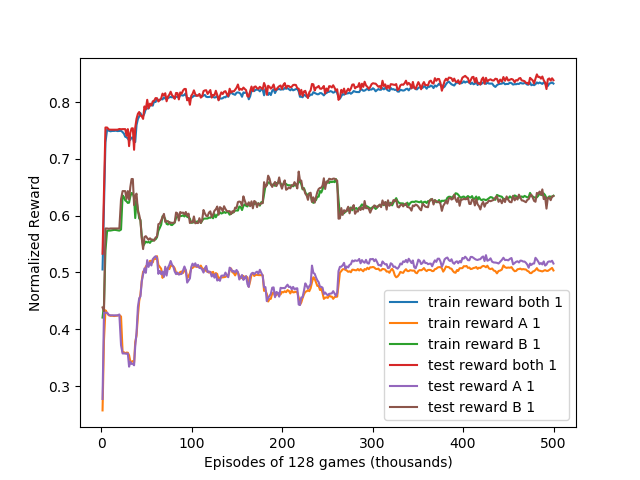
\includegraphics[width=0.9\linewidth]{opp-util-0.png}
    \end{center}
    %\caption{agent B knows A's utilities}
    \end{subfigure}%
    \begin{subfigure}{.5\textwidth}
    \begin{center}
        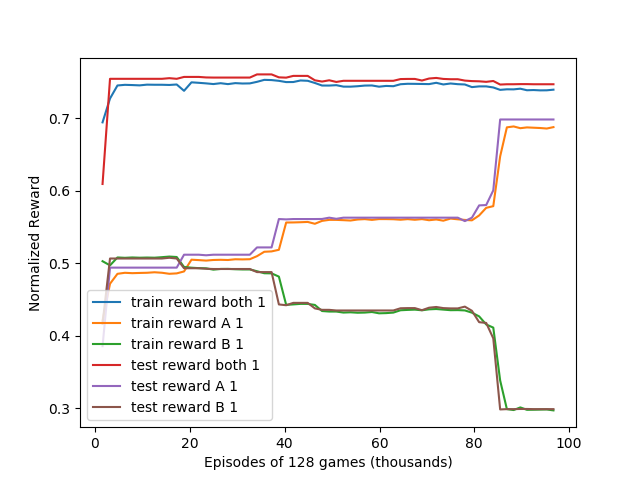
\includegraphics[width=0.9\linewidth]{opp-util-1.png}
    \end{center}
    %\caption{agent A knows B's utilities}
    \end{subfigure}
    \label{fig:self-opp-util}
    \caption{The agent that knows the other's utilities, dominates}
\end{figure}

\begin{table}[h]
    \centering
    \begin{tabular}{| c || c | c | }
        \hline
        \diagbox{Agent A}{Agent B} & Communicate & Don't Communicate \\
        \hline \hline
        Communicate & Equal & B dominates \\ \hline
        Don't Communicate & A dominates & Equal \\ \hline
    \end{tabular}
    \caption{payoff matrix for communicating utility as a selfish agent}
    \label{tab:payoff}
\end{table}

For selfish agents we
find that an agent tends to dominate its opponent if it knows the opponent's
preferences, and outcomes are relatively similar if neither agent knows the
opponent's preferences. This means that for selfish agents communicating their
utility as prosocial agents do can be described with the payoff matrix in table
\ref{tab:payoff}. In this way, selfish agents learn the optimal choice to not
communicate their utilities because they are disincentived to in this specific
situation.


\subsection{Equitable Reward Metric}%
\label{sub:equitable_reward_metric}
Since fractional reward is biased as explained in
\ref{sub:fractional_reward_is_biased}, a better metric for selfish agents is
proposed to measure the performance of their negotiation: equitable reward.
Since each agent's preferences may be at odds with the other, it is better to
measure the agents' performances taking into account a comparison of their
respective utilities. We consider optimality if each agent recieves a proportion
of the items in the pool corresponding to the fraction of their utility over
their utility and their opponents. Essentially, if each agent recieves items
according to how much they care about them:

\begin{equation}
    ER_{\text{selfish}} = \frac{u_A \cdot P}{(u_A + u_B) \cdot P}
\end{equation}

Since for any given $P$, for any selfish agents, $ER(A) + ER(B) = 1$, and since
we expect two random uniform policies to be equal in expectation, therefore we
expect both agents to perform with $ER ~ 0.5$ in expectation for them to be
performing fully equitably. This result is
found in running the selfish agent with just a proposal channel in
fig \ref{fig:self-prop} comparing the ER rewards (e.g. train reward A) with the
\textit{joint reward optimality} (e.g. train reward both)

\begin{figure}[h]
    \centering
    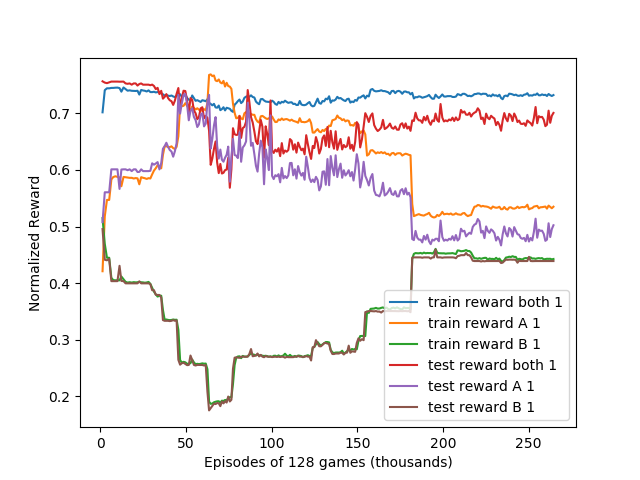
\includegraphics[width=0.8\linewidth]{self-prop.png}
    \caption{Selfish agents Using proposal channel}
    \label{fig:self-prop}
\end{figure}


\subsection{Utility Sampling}%
\label{sub:utility_sampling}
One consequence of randomly sampling utilities is that there is no
guarantee on the clash of utilities in negotation as the players could have
non-zero utility only for the items that their opponent has zero utility and
negotiation is simplified. To combat this issue, as identified in
\ref{sub:unmotivated_agents} it is proposed to guaranteee non-zero utility
to every item.

Another issue is that in the social case, one player's utilities could dominate
the other's $u_j^1 > u_j^2 \forall j$. In such a case, the optimal strategy for
both players is to give all items to the player with the dominating utility, and
again the player. The final split is therefore pareto optimal, but doesn't feel
"fair" for the side of the dominated player. A similar situation for a selfish
agent would generally lead to a more even split with a smaller total reward. For
this reason, we can experiment with avoiding domination situations by
normalizing the utilities so that each agents utilities all sum to 15.

\section{Conclusion}%
\label{sec:conclusion}

After thoroughly investigating the paper, we find certain flaws and extend the
work to cover them. Still, the main crux of the paper is that cooperation is
necessary for linguistic communication to emerge, and this thesis is not well
enough defended. We find that the experiments are biased towards prosocial
agents and through the setup deter selfish agents from communicating. In this
way, we find that it is not selfish agent failing to communicate but learning
specifically not to. For this reason, the idea that cooperation is necesary for
language is not thoroughly tested. Instead, it makes sense to reduce our
requirements and compare the idea of \cite{wittgenstein2009philosophical} that
it is not cooperation but opponent awareness that facilitates communication. For
this reason, we propose future work to investigate a model of selfish agents
that are incentivized to communicate to better understand their opponent,
without having the need to communicate with them.

\bibliography{report}
\bibliographystyle{plain}

\end{document}
